\section{Appendix}

\subsection{Dataset Statistics}

\begin{table}[h]
    \centering
    \caption{\textbf{Dataset Statistics.} The Table shows the number of samples and targets in each split of the two datasets.}
    \vspace{5pt}
    \label{tab:data}
    \begin{tabular}{lllll}
        \toprule
        & \textbf{Split} & \textbf{\#Samples} (\%) & \textbf{\#Targets} & \textbf{Overlap} \\
        \midrule
        \multirow{3}{*}{\texttt{TM}} 
        & Train. & 65,846 (62\%) & 59 & N/A \\
        & Val. & 15,031 (14\%) & 47 & 10 \\
        & Test. & 25,083 (24\%) & 37 & 4 \\
        \\
        \multirow{3}{*}{\texttt{SP}} 
        & Train. & 12,141 (85\%) & 636 & N/A \\
        & Val. & 1,407 (10\%) & 159 & 0 \\
        & Test. & 703 (5\%) & 89 & 0 \\
        \bottomrule
    \end{tabular}
\end{table}

\subsection{Way-Shot Analysis Heatmap}

\begin{figure}[h!]
    \centering
    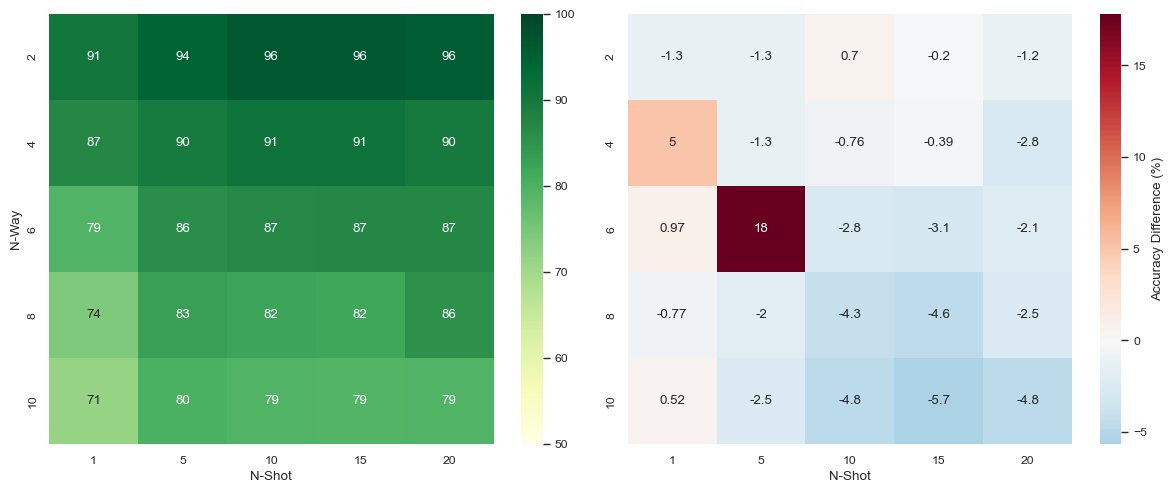
\includegraphics[width=1\columnwidth]{figures/way-shot-heatmap.png}
    \caption{\textbf{Way-Shot Analysis Heatmap.} Test accuracy of \texttt{PN} with SOT on the \texttt{TM} for varying numbers of classes and samples per class (left). The right plot shows the difference to the same method without SOT.}
    \label{fig:way-shot-heatmap}
\end{figure}
